%! TeX program = xelatex
\documentclass[../main.tex]{subfiles}

\begin{document}
\makelectureweek{9}{Week 9}

\section{Antiderivatives}

\begin{mdframed}[style=withref]
  \textbf{Definition}. Let \(f\) be a function. A function \(F\) is called an \emph{antiderivative} of \(f\) on an interval \(I\) if 
  \[
    {F'(x) = f(x) \text{ for all } x \text{ in } I.}
  \]

  \textbook{\stewart{357}{Definition}}
\end{mdframed}

\begin{example}
  Find an antiderivative of \(1/x\).
\end{example}
\vspace{1in}

\begin{example}
  Assume \(n \ne 1\). Find an antiderivative of \(x^{n}\).
\end{example}
\vspace{2in}

\begin{example}
  Is \(F(t) = \cos(t)\sin(t)\) an antiderivative of \(f(t) = -\sin(t)\cos(t)\)?

  % We want to find the antiderivative of \(f(t) = -\sin(t) \cos(t)\). Is the following reasoning correct?
  %
  % We know 
  % \begin{equation} \label{eq:wrong}
  %   \frac{d}{dt} \cos(t) = -\sin(t) \quad\text{and}\quad \frac{d}{dt} \sin(t) = \cos(t).
  % \end{equation} 
  %
  % Therefore, the antiderivative of \(-\sin(t)\) is \(\cos(t)\) and the antiderivative of \(\cos(t)\) is \(\sin(t)\).
  %
  % Because \(f(t)\) is the product of the right-hand sides of Equation~\eqref{eq:wrong}, we just take the product of their individual antiderivatives. 
  %
  % Therefore, the antiderivative of \(f(t)\) is
  % \[
  %   F(t) = \cos(t) \sin(t).
  % \]
\end{example}
\vspace{1in}

\clearpage
\begin{example} \label{ex:rock}
Assume all measurements are taken from the sea level.

A rock launched straight up with initial velocity \(2\) metres per second. The rock's vertical velocity function with respect to time is
\[
  v(t) = 2 - gt
\]
where \(g\) is the acceleration due to gravity.  We wish to find the height function \(h(t)\) of the rock. 

\faComment{} What is the relation between \(h(t)\) and \(v(t)\)?
\vspace{1in}

\faComment{} What are some possible expressions for \(h(t)\)?
\vspace{2in}

\faComment{} What is \emph{the most general} expression for \(h(t)\)?
\vspace{1in}
  
\end{example}
\begin{mdframed}[style=withref]
  \textbf{Theorem}. Let \(f\) be a function. If \(F\) is \emph{an} antiderivative of \(f\) on an interval \(I\), then \emph{the most general antiderivative} of \(f\) is
  \[
    F(x) + C
  \]
  where \(C\) is a symbol representing an arbitrary constant.

  \textbook{\stewart{357}{\fbox{1} Theorem}}
\end{mdframed}
\clearpage

\begin{example}
  We continue from Example~\ref{ex:rock}. Assume further that \(h(2) = 204\). Find the height function \(h(t)\).
\end{example}
\vspace{3in}

\begin{example}
  Find the function \(f\) if \(f'(x) = \sin(x) + e^{x} - \frac{1}{x}\) and \(f(1) = 3\).
\end{example}
\clearpage


Fill in the last column of Table~\ref{table:antiderivatives}.
\bigskip
\begin{table}[h!]
  \centering
  \includegraphics{../standalones/build/table_antiderivatives}
  \caption{Some well-known antiderivatives.}
  \label{table:antiderivatives}
\end{table}

\clearpage

\section{Sigma notation of summation}

The Sigma notation is a succint notation for adding a list of numbers.
\vspace{3in}

\begin{example}
  Expand the following summation in expanded forms.
  \bigskip

  \(\sum_{i=1}^{5} \sqrt[3]{i}\)
  \vspace{2cm}

  \(\sum_{j=3}^{5} (2j^{3} + 5^{j} + 1)\)
  \vspace{2cm}
  
  \(\sum_{k=10}^{15} x\)
  \vspace{2cm}
\end{example}

\clearpage

\begin{example}
  Express the \emph{total area} of the rectangles shown below in Sigma notation. The height of each rectangle is labelled on their top edge.

  \begin{center}
    \includegraphics{../standalones/build/plot_rectangles}
  \end{center}
\end{example}
\vfill

\clearpage
\begin{mdframed}[style=withref]
  \textbf{Theorem}. Let \(c\) be a constant. Let \(a_{1}, \dots, a_{n}, b_{1}, \dots, b_{n}\) be a list of numbers. We have
  \begin{align}
    \sum_{i=1}^{n} c a_{i} 
    &= c \sum_{i=1}^{n} a_{i} \\[2ex]
    \sum_{i=1}^{n} a_{i} + \sum_{i=1}^{n} b_{i} 
    &= \sum_{i=1}^{n} (a_{i} + b_{i}) \\[2ex]
    \sum_{i=1}^{n} a_{i} - \sum_{i=1}^{n} b_{i} 
    &= \sum_{i=1}^{n} (a_{i} - b_{i}).
  \end{align}

  \textbook{\stewart{A37}{\fbox{2} Theorem}}
\end{mdframed}

% \begin{example}
%   Let \(c\) be a constant. Let \(a_{1}, \dots, a_{n}, b_{1}, \dots, b_{n}\) be a list of numbers. 
%
%   Are the following equations true?
%   \begin{align}
%     \sum_{i=1}^{n} c a_{i} 
%     &= c \sum_{i=1}^{n} a_{i} \\[2ex]
%     \sum_{i=1}^{n} a_{i} + \sum_{i=1}^{n} b_{i} 
%     &= c \sum_{i=1}^{n} (a_{i} + b_{i}) \\[2ex]
%     \sum_{i=1}^{n} a_{i} - \sum_{i=1}^{n} b_{i} 
%     &= c \sum_{i=1}^{n} (a_{i} - b_{i}).
%   \end{align}
% \end{example}

\begin{example}
  Use the formula \(\sum_{i=1}^{n} i = \frac{n(n+1)}{2}\) to simplify \(\sum_{i=1}^{n}(2i + 1)\).
\end{example}
\clearpage

\begin{example}
  Use the formula \(\sum_{i=1}^{n} i^{2} = \frac{n(n+1)(2n+1)}{6}\) to evaluate \(\lim_{n \to \infty} \sum_{i=1}^{n} \frac{1}{n} \left( \frac{i}{n} \right)^{2}\).
\end{example}
\vfill
\clearpage

\section{The Area Problem}
Invent and \emph{explore} different \underline{methods} to \emph{approximate} the area (without units) of the bounded region with the following goals in mind:
\begin{enumerate}
  \item Your approximation can be expressed in Sigma notation. 
  \item The accuracy of your approximation can be improved.
  \item Your method works for other shapes. 
\end{enumerate}

% \begin{tikzpicture}
%
%   \begin{scope}[rotate=17.5]
%     \clip (4.5,-2) rectangle (17.5,9);
%     \node[opacity=1, above right] at (0,0) {\includegraphics[scale=0.8]{../standalones/map_campus}};
%   \end{scope}
%
%   \begin{scope}[rotate=17.5]
%     % help lines for clipping the photo
%     % \draw (0,-3) grid (18,10);
%     % \fill[red] (0,0) circle (5pt);
%
%     \begin{scope}[shift={(4,-2.5)}]
%       \draw[thick, white] (0,0) grid (14, 12);
%       \foreach \x in {1,...,13} {
%         \draw (\x, 0.05) -- (\x, -0.05) node[below] {\footnotesize \(\x\)};
%       }
%       \foreach \y in {1,...,11} {
%         \draw (0.05, \y) -- (-0.05, \y) node[left] {\footnotesize \(\y\)};
%       }
%
%       \begin{scope}[shift={(0,12)}]
%         \foreach \x in {1,...,13} {
%           \draw (\x, -0.05) -- (\x, 0.05) node[above] {\footnotesize \(\x\)};
%         }
%       \end{scope}
%       \begin{scope}[shift={(14,0)}]
%         \foreach \y in {1,...,11} {
%           \draw (-0.05, \y) -- (0.05, \y) node[right] {\footnotesize \(\y\)};
%         }
%       \end{scope}
%     \end{scope}
%   \end{scope}
%
% \end{tikzpicture}

\faComments{} \emph{How} can you do better than simply counting the number of squares inside the bounded region?

{\footnotesize{} See \href{}{FIXME (link here)} for a version where the map and the grid are plotted on separate pages.}
\vspace{1em}

\begin{tikzpicture}[x=1cm]
  \begin{scope}
    \clip (0,0) rectangle (15,15);
    %
    % no rotation (START HERE)
    %
    % \node[above right] at (0,0) {\includegraphics[width=14.7cm]{../standalones/map_campus}};

    % 
    % alinged at the bottom
    %
    \node[rotate={-17.5+180}] at (15/2+0.2, 15/2-2.5) {\includegraphics[width=14.7cm]{../standalones/map_campus}};
  \end{scope}

  % coarse grid
  % \draw[thick] (0,0) grid[step=1] (15,15);

  % finer grid
  \draw (0,0) grid[step=0.5] (15,15);

  % no grid
  % \draw (0,0) rectangle (15,15);

  \foreach \x in {1,...,15} {
    \draw (\x, 0.05) -- (\x, -0.05) node[below] {\footnotesize \(\x\)};
  }
  \foreach \y in {1,...,15} {
    \draw (0.05, \y) -- (-0.05, \y) node[left] {\footnotesize \(\y\)};
  }
\end{tikzpicture}
\clearpage

\begin{mdframed}[style=withref]
  The \emph{area} \(A\) that lies under the graph of a \emph{continuous} function \(f\) is the limit of sum of approximating rectangle:
  \vspace{1in}

  \textbook{\stewart{377}{\fbox{2} Definition}}
\end{mdframed}
\clearpage

\begin{example}
  Show the area under the curve \(y = x^{2}\) from \(a = 0\) to \(b = 1\) is \(1/3\). 

  \begin{tikzpicture}[scale=3]
    \begin{scope}
      \clip (-0.5,0) rectangle (1.5, 1.5);
      \draw[thick, dashed] plot[domain=-0.5:0] (\x, \x*\x);
      \draw[thick, teal] plot[domain=0:1] (\x, \x*\x);
      \draw[thick, dashed] plot[domain=1:1.5] (\x, \x*\x);
    \end{scope}
    \draw[very thin, ->] (-0.5,0) -- (1.2,0) node[right] {\footnotesize \(x\)};
    \draw[very thin, ->] (0,-0.2) -- (0,1.2) node[above] {\footnotesize \(y\)};
    \foreach \x in {1} {
      \draw (\x, 0.05) -- (\x, -0.05) node[below] {\footnotesize \(\x\)};
    }
    \foreach \y in {1} {
      \draw (0.05, \y) -- (-0.05, \y) node[left] {\footnotesize \(\y\)};
    }
  \end{tikzpicture}
\end{example}
\clearpage

In general, we have a lot of flexibility in choosing approximating rectangles.
\begin{mdframed}[style=withref]
  \vspace{1in}

  \textbook{\stewart{377}{\fbox{4}}}
\end{mdframed}

\vspace{1em}

Draw \(7\) approximating rectangles by choosing the sample points \(x_{i}^{*}\) to be the \emph{right endpoint} of the \(i\)-th subinterval.

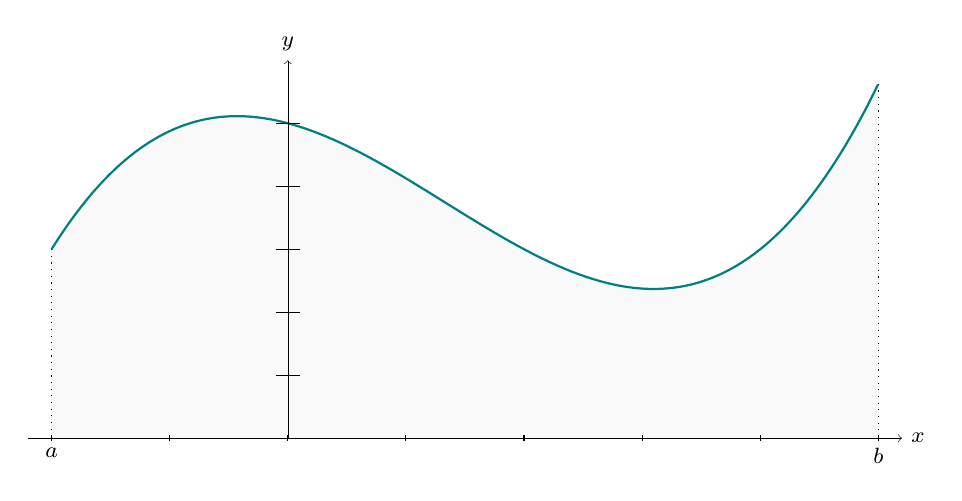
\begin{tikzpicture}[xscale=3,yscale=0.8]
  \begin{scope}
  \fill[gray!5] plot[domain=-1:2.5, samples=100, smooth] (\x, {(\x+1)*(\x-1)*(\x-2) + 3}) -- (2.5,0) -- (-1,0);
    \draw[dotted] (-1,3) -- (-1,0);
    \draw[dotted] (2.5, 5.625) -- (2.5, 0);
    \draw[thick, teal] plot[domain=-1:2.5, samples=100, smooth] (\x, {(\x+1)*(\x-1)*(\x-2) + 3});
    \node[below] at (-1,0) {\footnotesize \(a\)};
    \node[below] at (2.5,0) {\footnotesize \(b\)};
  \end{scope}

  \draw[very thin, ->] (-1.1,0) -- (2.6,0) node[right] {\footnotesize \(x\)};
  \draw[very thin, ->] (0,0) -- (0,6) node[above] {\footnotesize \(y\)};

  \foreach \x in {-1,-0.5,...,2.5} {
    \draw (\x, 0.05) -- (\x, -0.05); % node[below] {\footnotesize \(\x\)};
  }

  \foreach \y in {1,2,3,4,5} {
    \draw (0.05, \y) -- (-0.05, \y); % node[left] {\footnotesize \(\y\)};
  }
\end{tikzpicture}

Draw \(7\) approximating rectangles by choosing the sample points \(x_{i}^{*}\) to be the \emph{left endpoint} of the \(i\)-th subinterval.

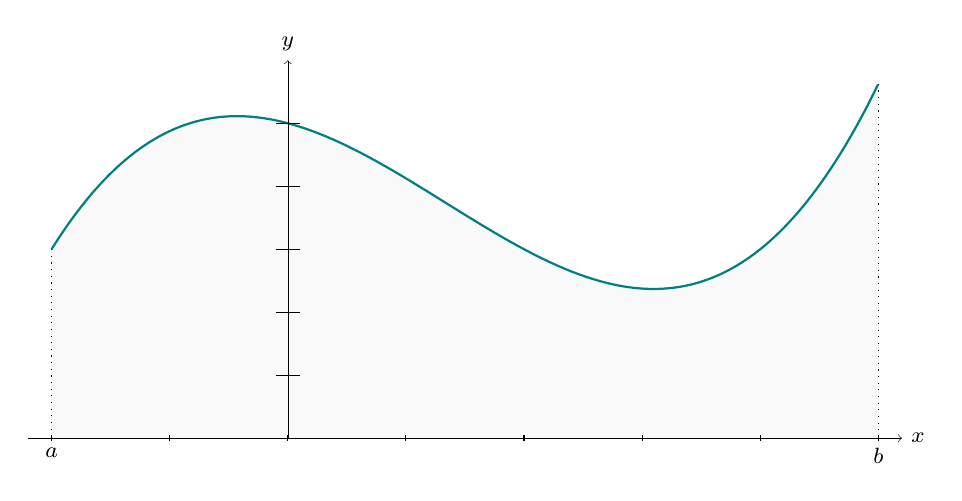
\begin{tikzpicture}[xscale=3,yscale=0.8]
  \begin{scope}
  \fill[gray!5] plot[domain=-1:2.5, samples=100, smooth] (\x, {(\x+1)*(\x-1)*(\x-2) + 3}) -- (2.5,0) -- (-1,0);
    \draw[dotted] (-1,3) -- (-1,0);
    \draw[dotted] (2.5, 5.625) -- (2.5, 0);
    \draw[thick, teal] plot[domain=-1:2.5, samples=100, smooth] (\x, {(\x+1)*(\x-1)*(\x-2) + 3});

    \node[below] at (-1,0) {\footnotesize \(a\)};
    \node[below] at (2.5,0) {\footnotesize \(b\)};
  \end{scope}

  \draw[very thin, ->] (-1.1,0) -- (2.6,0) node[right] {\footnotesize \(x\)};
  \draw[very thin, ->] (0,0) -- (0,6) node[above] {\footnotesize \(y\)};

  \foreach \x in {-1,-0.5,...,2.5} {
    \draw (\x, 0.05) -- (\x, -0.05); % node[below] {\footnotesize \(\x\)};
  }

  \foreach \y in {1,2,3,4,5} {
    \draw (0.05, \y) -- (-0.05, \y); % node[left] {\footnotesize \(\y\)};
  }
\end{tikzpicture}
\clearpage

Draw \(7\) approximating rectangles by choosing the sample points \(x_{i}^{*}\) to be the \emph{the midpoint} of the \(i\)-th subinterval.

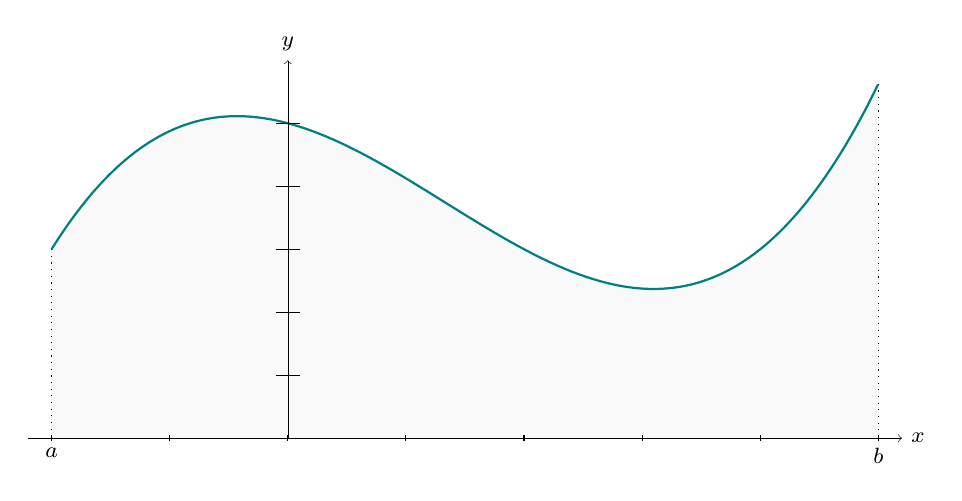
\begin{tikzpicture}[xscale=3,yscale=0.8]
  \begin{scope}
  \fill[gray!5] plot[domain=-1:2.5, samples=100, smooth] (\x, {(\x+1)*(\x-1)*(\x-2) + 3}) -- (2.5,0) -- (-1,0);
    \draw[dotted] (-1,3) -- (-1,0);
    \draw[dotted] (2.5, 5.625) -- (2.5, 0);
    \draw[thick, teal] plot[domain=-1:2.5, samples=100, smooth] (\x, {(\x+1)*(\x-1)*(\x-2) + 3});

    \node[below] at (-1,0) {\footnotesize \(a\)};
    \node[below] at (2.5,0) {\footnotesize \(b\)};
  \end{scope}

  \draw[very thin, ->] (-1.1,0) -- (2.6,0) node[right] {\footnotesize \(x\)};
  \draw[very thin, ->] (0,0) -- (0,6) node[above] {\footnotesize \(y\)};

  \foreach \x in {-1,-0.5,...,2.5} {
    \draw (\x, 0.05) -- (\x, -0.05); % node[below] {\footnotesize \(\x\)};
  }

  \foreach \y in {1,2,3,4,5} {
    \draw (0.05, \y) -- (-0.05, \y); % node[left] {\footnotesize \(\y\)};
  }
\end{tikzpicture}

Draw \(7\) approximating rectangles by choosing the samples points \(x_{i}^{*}\) so that \(f(x_{i}^{*})\) is the maximum value of \(f\) on the \(i\)-th subinterval.

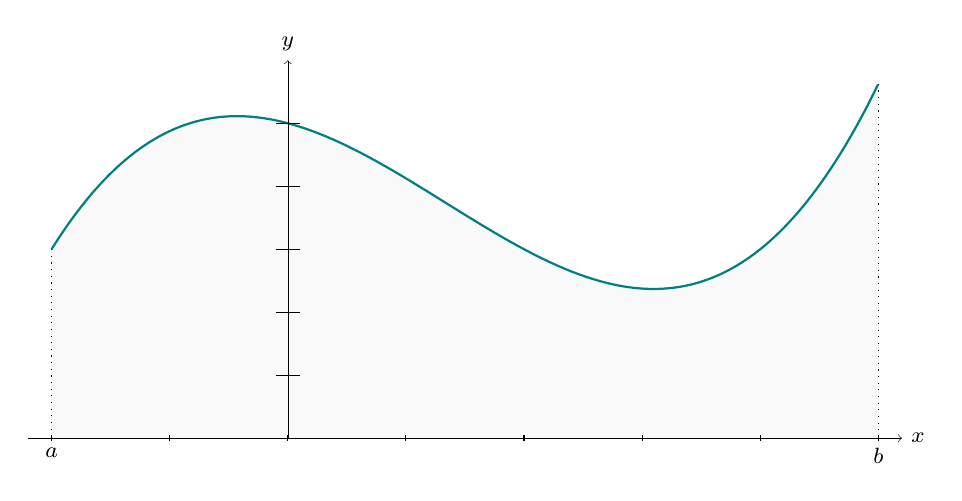
\begin{tikzpicture}[xscale=3,yscale=0.8]
  \begin{scope}
  \fill[gray!5] plot[domain=-1:2.5, samples=100, smooth] (\x, {(\x+1)*(\x-1)*(\x-2) + 3}) -- (2.5,0) -- (-1,0);
    \draw[dotted] (-1,3) -- (-1,0);
    \draw[dotted] (2.5, 5.625) -- (2.5, 0);
    \draw[thick, teal] plot[domain=-1:2.5, samples=100, smooth] (\x, {(\x+1)*(\x-1)*(\x-2) + 3});
    
    \node[below] at (-1,0) {\footnotesize \(a\)};
    \node[below] at (2.5,0) {\footnotesize \(b\)};
  \end{scope}

  \draw[very thin, ->] (-1.1,0) -- (2.6,0) node[right] {\footnotesize \(x\)};
  \draw[very thin, ->] (0,0) -- (0,6) node[above] {\footnotesize \(y\)};

  \foreach \x in {-1,-0.5,...,2.5} {
    \draw (\x, 0.05) -- (\x, -0.05); % node[below] {\footnotesize \(\x\)};
  }

  \foreach \y in {1,2,3,4,5} {
    \draw (0.05, \y) -- (-0.05, \y); % node[left] {\footnotesize \(\y\)};
  }
\end{tikzpicture}

Draw \(7\) approximating rectangles by choosing the samples points \(x_{i}^{*}\) so that \(f(x_{i}^{*})\) is the minimum value of \(f\) on the \(i\)-th subinterval.

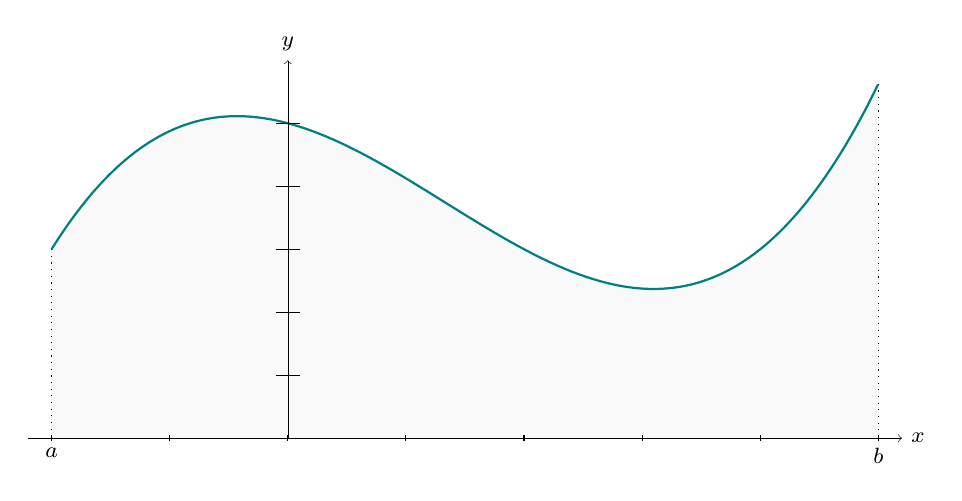
\begin{tikzpicture}[xscale=3,yscale=0.8]
  \begin{scope}
  \fill[gray!5] plot[domain=-1:2.5, samples=100, smooth] (\x, {(\x+1)*(\x-1)*(\x-2) + 3}) -- (2.5,0) -- (-1,0);
    \draw[dotted] (-1,3) -- (-1,0);
    \draw[dotted] (2.5, 5.625) -- (2.5, 0);
    \draw[thick, teal] plot[domain=-1:2.5, samples=100, smooth] (\x, {(\x+1)*(\x-1)*(\x-2) + 3});

    \node[below] at (-1,0) {\footnotesize \(a\)};
    \node[below] at (2.5,0) {\footnotesize \(b\)};
  \end{scope}

  \draw[very thin, ->] (-1.1,0) -- (2.6,0) node[right] {\footnotesize \(x\)};
  \draw[very thin, ->] (0,0) -- (0,6) node[above] {\footnotesize \(y\)};

  \foreach \x in {-1,-0.5,...,2.5} {
    \draw (\x, 0.05) -- (\x, -0.05); % node[below] {\footnotesize \(\x\)};
  }

  \foreach \y in {1,2,3,4,5} {
    \draw (0.05, \y) -- (-0.05, \y); % node[left] {\footnotesize \(\y\)};
  }
\end{tikzpicture}

\section{The Distance Problem}
The distance of an object travelling in a straight line at a \emph{constant} velocity can be computed by
\[
  \text{distance travelled} = (\text{constant velocity}) \times \text{time}.
\]
\faComments{} What does area has to do with this equation?
\vspace{1in}

\begin{example} \label{example:rock}
Assume we are on a planet where acceleration due to gravity is \(1\;m/s^{2}\). 

A rock is launched straight up with an initial velocity \(2\) metres per second. The rock's vertical velocity function with respect to time is
\[
  v(t) = 2 - t.
\]
Let \(h(t)\) be the height function of the rock. 
\bigskip

\faComments{} What is the physical interpretation of the area under the curve of \(v\) between \(t=0\) and \(t=2\)?

\includegraphics{../standalones/build/plot_rocket}

\faComments{} What does the area under the curve of \(v\) between \(t=0\) and \(t=2\) have to do with the height function \(h(t)\)? 
\end{example}

\clearpage
\begin{example}
  Approximate the area under the curve from \(t=0\) and \(t=1.5\) by subdividing the interval \([0,1.5]\) into \(3\) equal-width rectangles? Use the left endpoint approximation.

  You should get a number at the very end. 
\end{example}
\includegraphics{../standalones/build/plot_rocket}
\clearpage

\section{Preview of next week}
\begin{example}
  We continue from Example~\ref{example:rock}. Let's extend the domain of the velocity function \(v(t) = 2 - t\) to \([0,3]\). This function carries physical meaning. It says that the rock begins to fall after \(2\) seconds.

  \includegraphics{../standalones/build/plot_rocket_extended}

  \faComments{} What \emph{should} the shaded area mean in terms of distance and \(h(t)\)?
\end{example}
\end{document}
